\documentclass[aspectratio=169]{beamer}
\usetheme[faculty=phil]{fibeamer}
\usepackage{polyglossia}
\setmainlanguage{english} %% main locale instead of `english`, you
%% can typeset the presentation in either Czech or Slovak,
%% respectively.
\setotherlanguages{russian} %% The additional keys allow
%%
%%   \begin{otherlanguage}{czech}   ... \end{otherlanguage}
%%   \begin{otherlanguage}{slovak}  ... \end{otherlanguage}
%%
%% These macros specify information about the presentation
\title[AGLA2]{Analytical Geometry and Linear Algebra II, Lab 5} %% that will be typeset on the
\subtitle{Orthogonality + OrthoNormality + SO(3) \\ Gram-Schmidt \\ Preparation to midterm 
         } %% title page.
\author{Oleg Bulichev}
%% These additional packages are used within the document:
\usepackage{ragged2e}  % `\justifying` text
\usepackage{booktabs}  % Tables
\usepackage{tabularx}
\usepackage{tikz}      % Diagrams
\usetikzlibrary{calc, shapes, backgrounds}
\usepackage{amsmath, amssymb}
\usepackage{url}       % `\url`s
\usepackage{listings}  % Code listings
% \usepackage{subfigure}
\usepackage{floatrow}
\usepackage{subcaption}
\usepackage{mathtools}
\usepackage{todonotes}
\usepackage{fontspec}
\usepackage{multicol}
\usepackage{pdfpages}
\usepackage{wrapfig}
\usepackage{animate}

\graphicspath{{resources/}}
\frenchspacing

\setbeamertemplate{caption}[numbered]
\usetikzlibrary{graphs}

% \usepackage[backend=biber,style=ieee,autocite=footnote]{biblatex}
% \addbibresource{biblio.bib}
% \DefineBibliographyStrings{english}{%
%   bibliography = {References},}

\newcommand{\oleg}[2][] {\todo[color=red, #1] {OLEG:\\ #2}}
\newcommand{\fbckg}[1]{\usebackgroundtemplate{\includegraphics[width=\paperwidth]{#1}}}%frame background

\usepackage[framemethod=TikZ]{mdframed}
\newcommand{\dbox}[1]{
\begin{mdframed}[roundcorner=3pt, backgroundcolor=yellow, linewidth=0]
\vspace{1mm}
{#1}
\vspace{1mm}
\end{mdframed}
}

\begin{document}
\setlength{\abovedisplayskip}{0pt}
\setlength{\belowdisplayskip}{0pt}
\setlength{\abovedisplayshortskip}{0pt}
\setlength{\belowdisplayshortskip}{0pt}

\fbckg{fibeamer/figs/title_page.png}
\frame[c]{\setcounter{framenumber}{0}
    \usebeamerfont{title}%
    \usebeamercolor[fg]{title}%
    \begin{minipage}[b][6.5\baselineskip][b]{\textwidth}%
        \textcolor{black}{\raggedright\inserttitle}
    \end{minipage}
    % \vskip-1.5\baselineskip

    \usebeamerfont{subtitle}%
    \usebeamercolor[fg]{framesubtitle}%
    \begin{minipage}[b][3\baselineskip][b]{\textwidth}
        \raggedright%
        \insertsubtitle%
    \end{minipage}
    \vskip.25\baselineskip
}
%   \frame[c]{\maketitle}

\fbckg{fibeamer/figs/common.png}

% \begin{frame}[c]{How I spent last weekend}
%     \framesubtitle{}
%     \begin{figure}[H]
%         \begin{subfigure}{0.49\textwidth}
%             \centering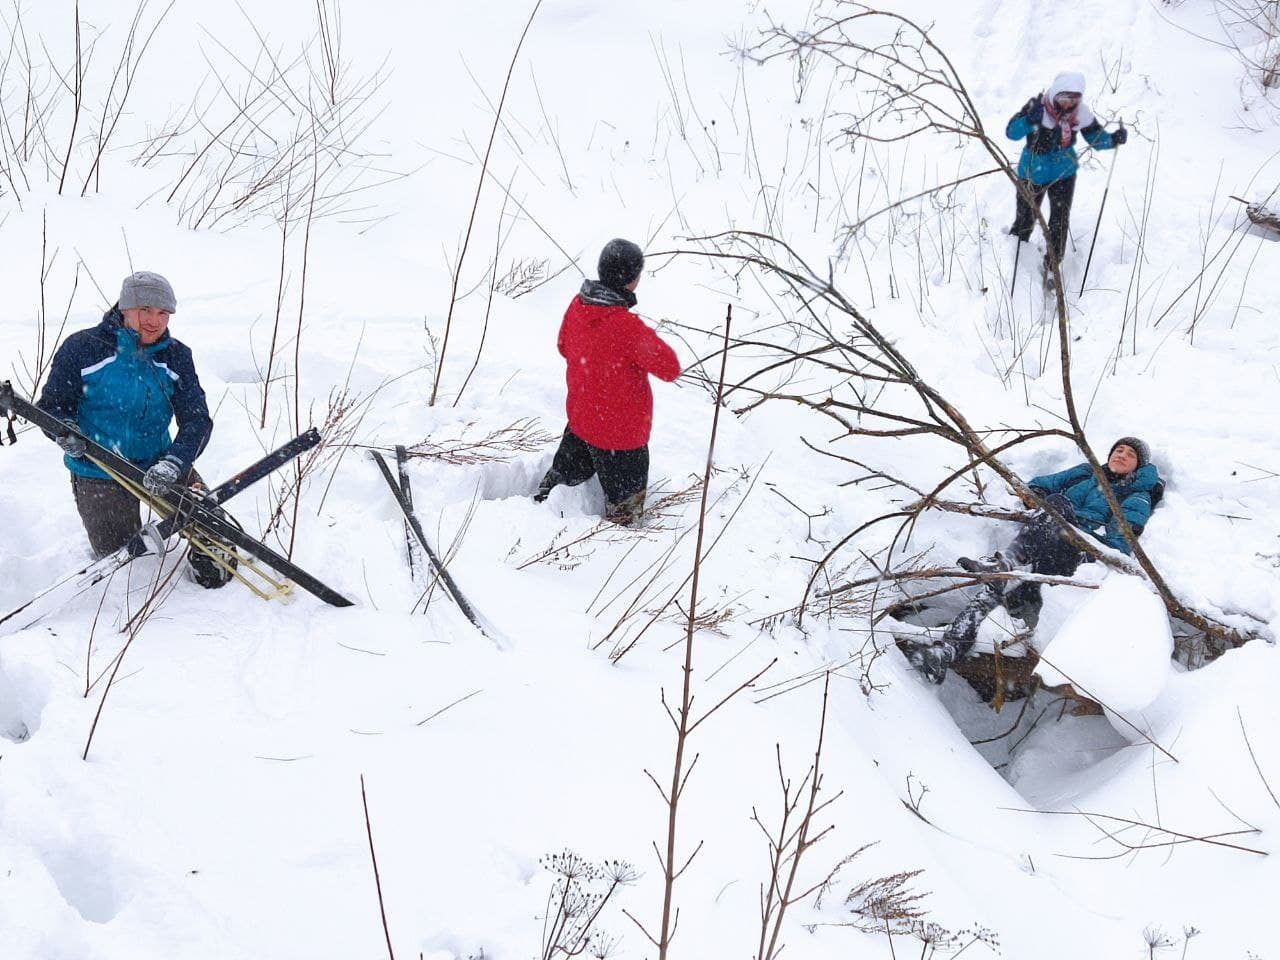
\includegraphics[height=5cm,width=1\textwidth,keepaspectratio]{skate-skiing.jpg}
%             \caption{Cross-country skiing}
%             \label{fig:file_name1}
%         \end{subfigure}
%         \begin{subfigure}{0.49\textwidth}
%             \centering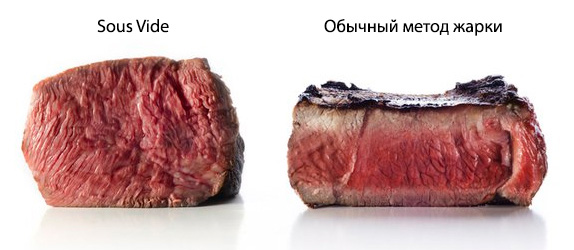
\includegraphics[height=5cm,width=1\textwidth,keepaspectratio]{sous_vide.jpg}
%             \caption{Sous vide}
%             \label{fig:file_name2}
%         \end{subfigure}

%         % \caption{capture_main}
%         % \label{fig:}
%     \end{figure}
% \end{frame}


\begin{frame}[t]{Orthogonality + OrthoNormality}
    \framesubtitle{}
    \vspace{-0.4cm}
    \renewcommand{\baselinestretch}{0.1}

    \begin{columns}[T,onlytextwidth]
        \begin{column}{0.49\textwidth}
            \begin{minipage}{0.58\textwidth}
                \begin{tikzpicture}
                    \draw[thick, ->, red] (0,0) -- (3,0);
                    \draw[thick, ->, red] (0,0) -- (1,2.5);
                    \draw[ultra thick, ->, blue] (0,0) -- (3,2.5);
                    \draw[dashed] (3,0) -- (3,2.5) -- (1,2.5);
                \end{tikzpicture}
            \end{minipage}\hfill
            \begin{minipage}{0.40\textwidth}
                \centering\textbf{Common}
                \begin{align*}
                    a \cdot b \neq 0 \\
                    b \cdot c \neq 0 \\
                    a \cdot c \neq 0 \\
                    \|a\|,\ \|b\|,\ |c\| \neq 1
                \end{align*}
            \end{minipage}

            \begin{minipage}{0.58\textwidth}
                \begin{tikzpicture}
                    \draw[thick, ->, red] (0,0) -- (3,0);
                    \draw[thick, ->, red] (0,0) -- (0,1);
                    \draw[ultra thick, ->, blue] (0,0) -- (3,2.5);
                    \draw[dashed] (3,0) -- (3,2.5) -- (0,2.5) -- (0,1);
                \end{tikzpicture}
            \end{minipage}\hfill
            \begin{minipage}{0.40\textwidth}
                \centering\textbf{Orthogonal}
                \begin{align*}
                    a \cdot b = 0 \\
                    b \cdot c = 0 \\
                    a \cdot c = 0 \\
                    \|a\|,\ \|b\|,\ |c\| \neq 1
                \end{align*}
            \end{minipage}
        \end{column}
        \begin{column}{0.49\textwidth}
            \begin{minipage}{0.58\textwidth}
                \begin{tikzpicture}
                    \draw[thick, ->, red] (0,0) -- (1,0);
                    \draw[thick, ->, red] (0,0) -- (0,1);
                    \draw[ultra thick, ->, blue] (0,0) -- (3,2.5);
                    \draw[dashed] (1,0) -- (3,0) -- (3,2.5) -- (0,2.5) -- (0,1);
                \end{tikzpicture}
            \end{minipage}\hfill
            \begin{minipage}{0.40\textwidth}
                \centering\textbf{OrthoNormal}
                \begin{align*}
                    a \cdot b = 0            \\
                    b \cdot c = 0            \\
                    a \cdot c = 0            \\
                    \|a\|,\ \|b\|,\ |c\| = 1 \\
                    det= \pm 1
                \end{align*}
            \end{minipage}
            \centering \textbf{Properties of orthogonal matrices} \\ {\centering (if they are square)}
            \begin{align*}
                Q^T=Q^{-1},\ \text{case study} \rightarrow \text{rotation matrix} \\
                \text{Orthogonal matrix }\rightarrow \ Q^TQ = I \\
                \text{Not normalized } Q \rightarrow \ N^TN = Diag
            \end{align*}
        \end{column}
    \end{columns}
\end{frame}

\begin{frame}[t]{Special orthonormal group (SO(n)) group}
    \framesubtitle{}
    \begin{figure}[H]
        \href{https://disk.yandex.ru/i/XD6o-ZIGS4yLvA}{\centering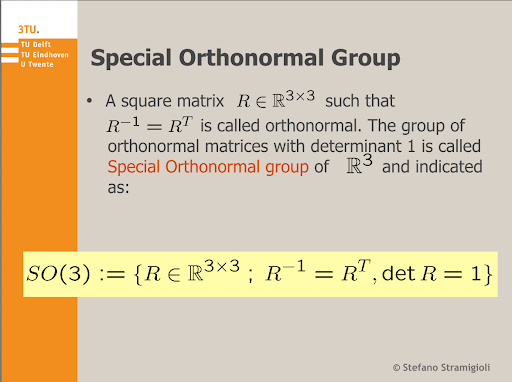
\includegraphics[height=5cm,width=1\textwidth,keepaspectratio]{course_modern.png}}
        \caption*{Modern robotics course, 1 lec (math background, LA + phys + advanced stuff for self education)}
        \label{fig:course_modern.png}
    \end{figure}
\end{frame}

\begin{frame}[t]{Gram-Schmidt}
    \framesubtitle{Summary}
    \Large
    This approach provides to \textbf{change} our \alert{common basis} to \alert{orthonormal basis} (our basis will have another vectors, but it represents the same (sub)space).

    If we \textbf{had vectors in old basis before}, we should find the linear combination values again \textbf{by solving system of linear equations}.

\end{frame}

\begin{frame}[t]{Gram-Schmidt}
    \framesubtitle{Algorithm}
    \vspace{-0.8cm}
    \centering 
    \animategraphics[height=6.2cm,autoplay,controls]{10}{gram_schmidt_animation/gram_}{1}{153}
\end{frame}


\usebackgroundtemplate{}
\setbeamercolor{background canvas}{bg=}
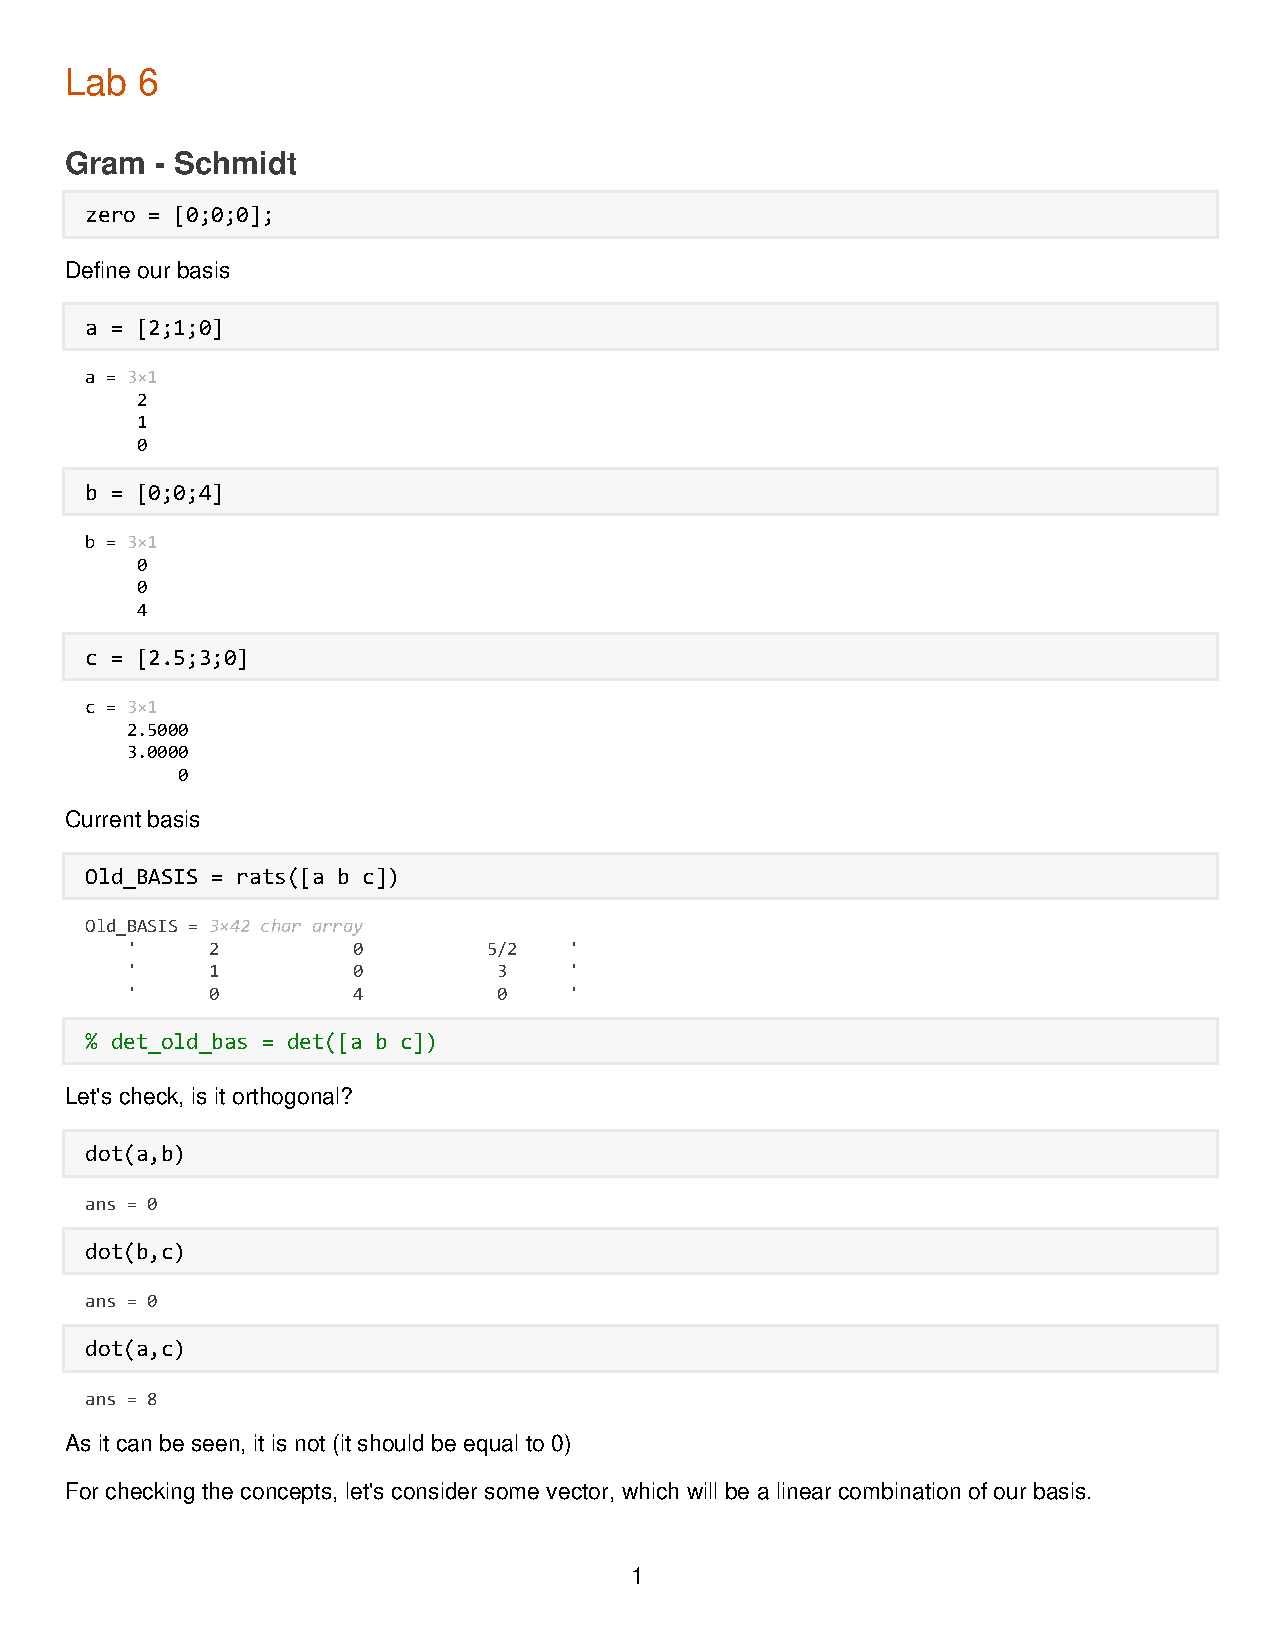
\includepdf[pages=-,fitpaper]{lab6_Gram_Schmidt.pdf}
\fbckg{fibeamer/figs/common.png}


\begin{frame}[t]{Gram-Schmidt}
    \framesubtitle{Task 1}
    \vspace{-0.2cm}
    \uncover<1->{Consider a subspace of all four-by-one column vectors with the following basis:
        \begin{equation*}W =
            \begin{bmatrix}
                1 & 0 & 0 \\
                1 & 1 & 0 \\
                1 & 1 & 1 \\
                1 & 1 & 1 \\
            \end{bmatrix}
        \end{equation*}
        \vspace{-0.3cm}
        \begin{enumerate}
            \item Use the Gram-Schmidt process to construct an orthogonal basis for this subspace.
            % \item We have coordinates of a vector $\vec{x}=\begin{bmatrix}
            %               2 \\
            %               3 \\
            %               1 \\
            %               1
            %           \end{bmatrix}
            %       $ in old basis. Find the scalar values witch provide us the same vector in new basis.
        \end{enumerate}
    }
    \uncover<2->{\alert{\Large Answers}
        \begin{enumerate}
            \item $W_{new} = \begin{bmatrix}
                          1 & -\frac{3}{4} & 0            \\
                          1 & \frac{1}{4}  & -\frac{2}{3} \\
                          1 & \frac{1}{4}  & \frac{1}{3}  \\
                          1 & \frac{1}{4}  & \frac{1}{3}  \\
                      \end{bmatrix}$ - \alert{Not normalized!!}
            % \item Linear combination is $\begin{bmatrix}
            %               \frac{7}{4}  \\
            %               -\frac{1}{3} \\
            %               -2
            %           \end{bmatrix}$
        \end{enumerate}

    }
\end{frame}

\begin{frame}[t]{QR Factorization}
\framesubtitle{}
\vspace{-0.8cm}
    \begin{columns}[T,onlytextwidth]
        \begin{column}{0.49\textwidth}
            \begin{figure}[H]
                \centering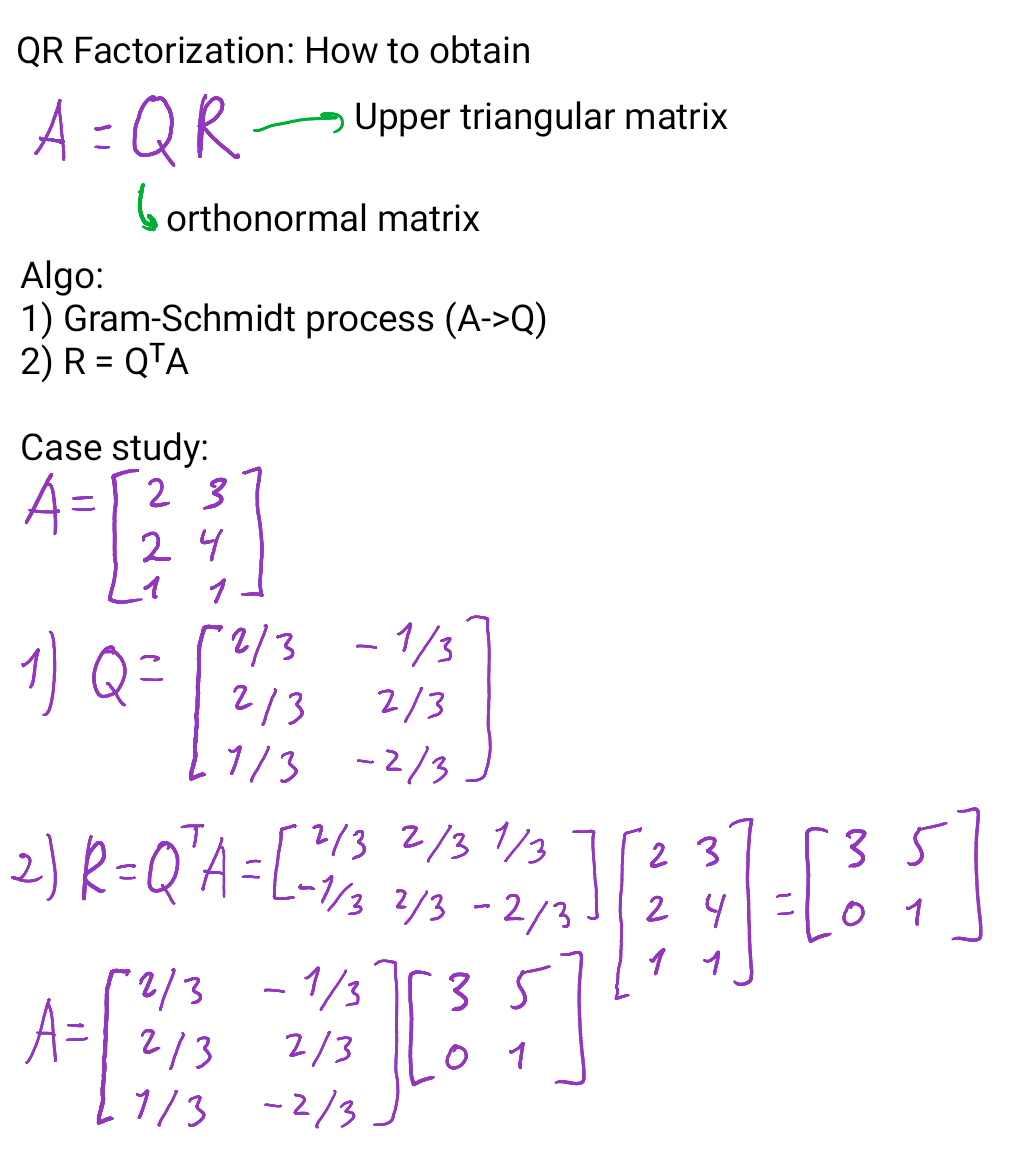
\includegraphics[height=6.5cm,width=1\textwidth,keepaspectratio]{AGLA2_for_slides_7.png}
                % \caption{caption_name}
                \label{fig:AGLA2_for_slides_7.png}
            \end{figure}    
        \end{column}
        \begin{column}{0.49\textwidth}
            \begin{figure}[H]
                \centering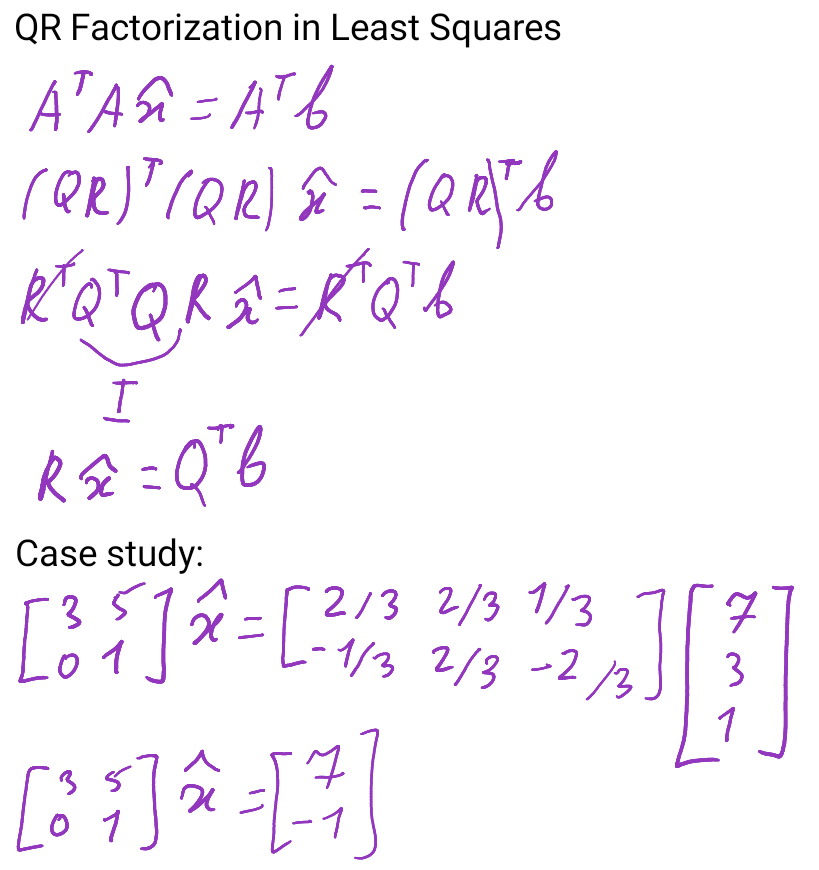
\includegraphics[height=6.5cm,width=1\textwidth,keepaspectratio]{AGLA2_for_slides_8.png}
                % \caption{caption_name}
                \label{fig:AGLA2_for_slides_8.png}
            \end{figure}    
        \end{column}
    \end{columns}
\end{frame}

\begin{frame}[t]{Quiz}
    \framesubtitle{}
    \only<1>{
        \textbf{\Large Tasks:}
        \begin{enumerate}
            \item \textit{Least Squares}. There are several points
                  $A = \begin{bmatrix}-1\\2\end{bmatrix};\
                      B = \begin{bmatrix}1\\0\end{bmatrix};\
                      C = \begin{bmatrix}-1\\0\end{bmatrix};\
                      D = \begin{bmatrix}2\\1\end{bmatrix};\
                      E = \begin{bmatrix}0\\-1\end{bmatrix};\
                      F = \begin{bmatrix}1\\2\end{bmatrix}.
                  $
                  \begin{enumerate}
                      \item What curve type is the best for fitting these points? (no more than 2nd order polynomial eq.)
                      \item Find the parameters of the curve, find summary error (SE).
                  \end{enumerate}
            \item \textit{Gram-Schmidt}. There is a basis $\begin{bmatrix}
                          14  & 3 & -1 & -1 \\
                          21  & 0 & 0  & 2  \\
                          14  & 0 & 2  & -1 \\
                          -14 & 3 & 1  & 1
                      \end{bmatrix}$. Make this basis orthogonal.
        \end{enumerate}
    }
    \only<2>{
        \alert{\Large Answers}
        \begin{columns}[T,onlytextwidth]
            \begin{column}{0.49\textwidth}
                \begin{enumerate}
                    \item \textit{Least Squares}
                          \begin{enumerate}
                              \item Parabola (or any 2nd order polynomial curve)
                              \item $a = 0.4,\ b=-0.2,\ c = 0.2;\ SE = 6.4$
                          \end{enumerate}
                    \item \textit{Gram-Schmidt}
                          \begin{enumerate}
                              \item The same. It is already orthogonal \heartsuit
                          \end{enumerate}
                \end{enumerate}
            \end{column}
            \begin{column}{0.49\textwidth}
                \vspace{-1.2cm}
                \begin{figure}[H]
                    \centering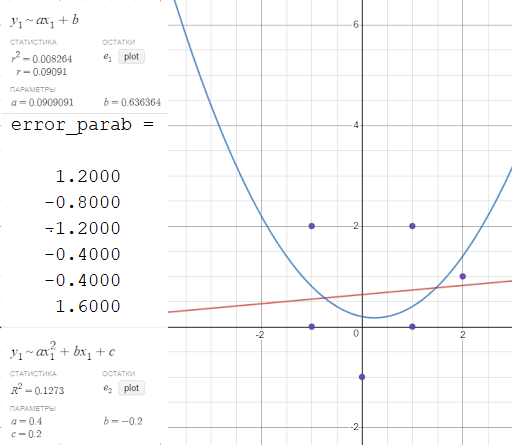
\includegraphics[height=5.5cm,width=1\textwidth,keepaspectratio]{quiz_ans.png}
                    \caption*{\Large Task 1}
                    \label{fig:quiz_ans}
                \end{figure}
            \end{column}
        \end{columns}
    }
\end{frame}

\begin{frame}[t]{Task 1}
    \framesubtitle{Midterm Preparation}
    \textbf{Task:} find $v$, where $v$ is intersection of $
        \left\{\begin{matrix*}[l]
            S_1 = x+7y-3z=13\\
            S_2=x+y+0z=5
        \end{matrix*}\right.
    $

    \uncover<2->{
        \alert{\Large Answer}
        \begin{enumerate}
            \item Using line representation as an intersection between two planes (AGLA1, lab 7).
            \item Using knowledge about solving undetermined equations (AGLA2, lab 3).
        \end{enumerate}
    }
\end{frame}

\begin{frame}[t]{Task 2}
    \framesubtitle{Midterm Preparation}
    \textbf{Task:} Find a vector $v$ that is orthogonal to $S$, if subspace $S$ of $R^3$ is formed by linear combination of vectors $v_1 = \begin{bmatrix}1\\2\\1\end{bmatrix}$ and $v_2 = \begin{bmatrix}2\\4\\2\end{bmatrix}$

    \uncover<2->{
        \alert{\Large Answer}
        \begin{enumerate}
            \item Using knowledge about projection (AGLA2, lab 5).
            \item Using knowledge that nullspace perpendicular to row space (AGLA2, lab 4).
        \end{enumerate}
    }
\end{frame}

\begin{frame}[t]{Task 3}
    \framesubtitle{Midterm Preparation}
    \only<1>{
        \textbf{Task:}
        \begin{enumerate}
            \item For each real parameter $\lambda$ construct a linear independent system that contains the maximum number of the following vectors.
            \item Find the dimensions of the four fundamental subspaces associated with result of "1", depending on the parameter $\lambda$.
        \end{enumerate}
        \begin{equation*}
            a=\begin{bmatrix}-\lambda\\1\\2\\3\end{bmatrix};\ b=\begin{bmatrix}1\\-\lambda\\3\\2\end{bmatrix};\ c=\begin{bmatrix}2\\3\\-\lambda\\1\end{bmatrix};\ d=\begin{bmatrix}3\\2\\1\\-\lambda\end{bmatrix};\ e=\begin{bmatrix}1\\1\\1\\1\end{bmatrix}.
        \end{equation*}
    }
    \only<2>{
        \begin{columns}[T,onlytextwidth]
            \begin{column}{0.64\textwidth}
                \alert{\Large Answer:} $\vec{a}$, $\vec{b}$, $\vec{c}$, $\vec{d}$, when $\lambda \neq 6$.
                \begin{enumerate}
                    \item Using \textbf{rref} we can easily find max possible max rank, hence choose our basis.

                          \textit{Hint}: It can be solved, if you sum all vectors to the first column (all rows will be the same).
                    \item Using knowledge from previous lab (AGLA2, lab 4).
                \end{enumerate}

            \end{column}
            \begin{column}{0.35\textwidth}
                \vspace{-0.3cm}
                \begin{figure}[H]
                    \centering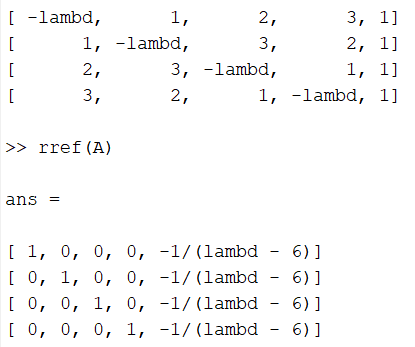
\includegraphics[height=4cm,width=1\textwidth,keepaspectratio]{task3_ans.png}
                    % \caption{caption_name}
                    \label{fig:task3_ans.png}
                \end{figure}
            \end{column}
        \end{columns}

    }
\end{frame}

\begin{frame}[t]{Reference material}
    \framesubtitle{}
    \Large
    \begin{itemize}
        \item \href{https://www.youtube.com/watch?v=Y_Ac6KiQ1t0&list=PL49CF3715CB9EF31D&index=17}{Lecture 17}
        \item \textit{"Linear Algebra and Applications", pdf pages 205--221 }\\ Orthogonal Bases and Gram-Schmidt
        \item \href{https://www.youtube.com/watch?v=eib8uAlzegc&list=PLkZjai-2Jcxlg-Z1roB0pUwFU-P58tvOx&index=20}{Gram-Schmidt Process | Lectures 19 and 20}\\ Video from Matrix Algebra for Engineers course
        \item \href{https://www.youtube.com/watch?v=J41Ypt6Mftc}{QR Factorization}
    \end{itemize}
\end{frame}

\fbckg{fibeamer/figs/last_page.png}
\frame[plain]{}

\end{document}